\documentclass{article}
\usepackage{fontspec}
\pagestyle{empty}
\usepackage{geometry}
\geometry{paperwidth=80mm, paperheight=80mm, left=2mm, top=0mm, right=2mm, bottom=0mm}
\parindent=0pt
\usepackage{color}
\usepackage{xcolor}
\usepackage{tikz}


\begin{document}
\centering
\vspace*{\fill} \vspace*{-5ex}

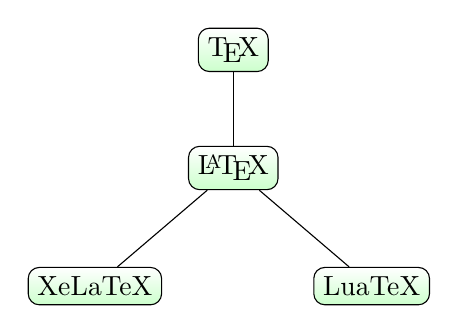
\begin{tikzpicture}[sibling distance=10em,
  every node/.style = {shape=rectangle, rounded corners,
    draw, align=center,
    top color=white, bottom color=green!20}]]
  \node {\TeX}
    child { node {\LaTeX}
      child { node {XeLaTeX} }
      child { node {LuaTeX} }
      } ;
\end{tikzpicture}
\vspace*{\fill} 
\end{document}